\subsection{Glyph: \glyph{Or}}
\label{sec:or}

The output of an \glyph{or} glyph is True if at least one of its inputs is True, and False otherwise.

\begin{glyphDescription}

\glyphSboTerm
SBO:0000174 ! or

\glyphIncoming One or more \glyph{logic arcs} (\sect{logicArc}).

\glyphOutgoing
One \glyph{logic arc} (\sect{logicArc}) or \glyph{modulation arc} (\sect{modulations}).

\glyphContainer
An \glyph{or} operator is represented by a circular shape containing the word ``OR''.
The shape is linked to two ports, that are small arcs attached to the centres of opposite sides of the shape, as shown in \fig{or}.
The incoming \glyph{logic arcs} (\sect{logicArc}) are linked to the extremity of the leftmost or uppermost port, while the outgoing \glyph{logic arc} (\sect{logicArc}) or \glyph{modulation} (\sect{modulation}) is linked to the extremity of the rightmost or bottommost port.

\glyphLabel
\corr{An \glyph{or} operator is not identified by any label}{None}.

\glyphAux
\corr{An \glyph{or} operator does not carry any auxiliary items}{None}.

\end{glyphDescription}

\begin{figure}[H]
  \centering
  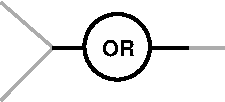
\includegraphics{images/build/or.pdf}
  \caption{The \PD glyph for \glyph{or}. Only two inputs are represented, but more would be allowed.}
  \label{fig:or}
\end{figure}

